\documentclass[a4paper,11pt]{article}

\usepackage[utf8]{inputenc}
\usepackage[T1]{fontenc}
\usepackage[french]{babel}
\usepackage{amsmath,amssymb}
\usepackage{fullpage}
\usepackage{xspace}
\usepackage{graphicx}
\usepackage{verbatim}
\usepackage{listings}
\usepackage[usenames,dvipsnames]{xcolor}
\usepackage{url}

\newtheorem{question}{Question}
\newtheorem{exo}{Exercice}

\newcommand{\dx}{\,dx}
\newcommand{\ito}{,\dotsc,}
\newcommand{\R}{\mathbb{R}}
\newcommand{\C}{\mathbb{C}}
\newcommand{\N}{\mathbb{N}}
\newcommand{\Poly}[1]{\mathcal{P}_{#1}}
\newcommand{\abs}[1]{\left\lvert#1\right\rvert}
\newcommand{\norm}[1]{\left\lVert#1\right\rVert}
\newcommand{\pars}[1]{\left(#1\right)}
\newcommand{\bigpars}[1]{\bigl(#1\bigr)}
\newcommand{\set}[1]{\left\{#1\right\}}

\title{Stage de Toussaint Ensimag 1A \\ Compte-rendu TP Scilab/Latex}
\author{Maxime Gourgoulhon \and Julie Saouli}
\date{Novembre 2016}

\begin{document}

\maketitle

%TODO
% renommer les scripts
% exercice 2 script + comm / exercice 3 q2 !! + comm
% exercice 4 comm
% exercice 6 graphes + comm
% exercice 7 graphe q3
% relecture globale

\section{Sensibilisation à l'arithmétique machine}

\subsection*{Exercice 1}
	En exécutant les commandes données dans Scilab, on obtient :
	\begin{verbatim}
	--> z = 0.
	--> w = 1.
	\end{verbatim}
	
	Dans le calcul de z, comme $x >> y$, y est négligé devant x dans l'addition de ces deux valeurs. De ce fait, $(y+x)-x \simeq x - x = 0$.
	Dans le calcul de w, les parenthèses évitent ce problème car toutes les opérations sont effectuées entre des termes de même ordre ou avec 0.
	
	
\subsection*{Exercice 2}
\begin{figure}[!h]
	\begin{center}
		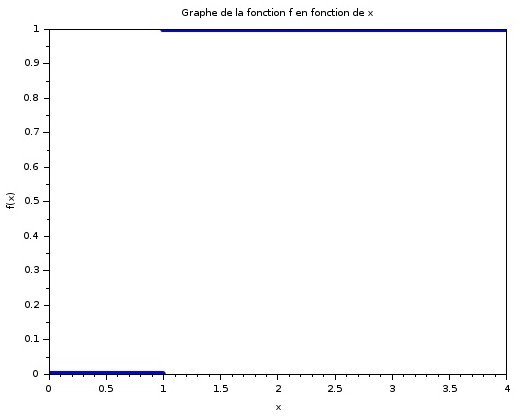
\includegraphics[scale=0.5]{graphes/exercice2.jpg}
		\caption{Graphe de la fonction $f$ en fonction de $x \in [0,4]$.}
	\end{center}	
\end{figure}

	D'après le graphe, on constate que $\forall x \in [0, 1]$ $f(x) = 0$.

\subsection*{Exercice 3}
	1. On commence par calculer les premiers termes de la suite $I_{n} = \int_0^1 x^{n} e^{x} dx$.
	\begin{align*}
		& I_{0} = \int_0^1 e^{x} dx = [e^{x}]_0^1 = e - 1 \\
		& I_{1} = \int_0^1 x e^{x} dx = [x e^{x}]_0^1 - I_{0} = e - I_{0} = 1 \\
		& I_{2} = \int_0^1 x^{2} e^{x} dx = [x^{2} e^{x}]_0^1 - 2I_{1} = e - 2I_{1} e - 2
	\end{align*}

	On en déduit la relation suivante : $I_{n} = e - nI_{n-1}$, que l'on vérifie par récurrence :
	\begin{equation*}
		I_{n+1} = \int_0^1 x^{n+1} e^{x} dx = [x^{n+1} e^{x}]_0^1 - (n+1) I_{n} = e - (n+1)I_{n}
	\end{equation*}

	Avec Scilab on évalue $I_{20}$.
	%partie scilab : calculer I20 à partir de I0 + constat

	2. On cherche maintenant à évaluer $I_{20}$ par un développement en série entière de $e^{x}$.
	\begin{equation*}
		I_{20} = \int_0^1 x^{20} e^{x} dx
		= \int_0^1 x^{n} \sum_{n=0}^{+\infty} \frac{x^{n}}{n!} dx
		= \sum_{n=0}^{+\infty} \frac{1}{n!} \int_0^1 x^{n+20} dx
		= \sum_{n=0}^{+\infty} \frac{1}{(n+21)n!}
	\end{equation*}
	Avec Scilab on évalue à nouveau $I_{20}$ mais avec cette nouvelle formule.
	%idem que autre méthode
	
	3. %conclusion

\subsection*{Exercice 4}
	Le script associé à cet exercice est nommé \textit{exercice4.sce}. Pour $n$ suffisamment grand, on retrouve bien le même résultat qu'à l'exercice 3.2.
	% quand on aura trouvé I20 avec le DL en série, donner un exemple de n

\section{Étude du phénomène de Gibbs}

\subsection*{Exercice 5}
	On cherche à calculer la série de Fourier de $f$. On remarque que $f$ est impaire donc $\forall n \in \mathbb{N} $ $a_{n}(f) = 0$.
	On commence par calculer $b_{n}(f)$ $\forall n \in \mathbb{N}^{*}$ :
	\begin{align*}
		b_{n}(f)
		& = 2 \int_{-\frac{1}{2}}^{\frac{1}{2}} f(t) \sin (2 \pi n t) dt \\
		& = 2 \left ( - \int_{-\frac{1}{2}}^{0} \sin (2 \pi n t) dt + \int_{0}^{\frac{1}{2}} \sin (2 \pi n t) dt \right ) \\
		& = 2 \left ( \left [ \frac{\cos ( 2 \pi n t)}{2 \pi n} \right ]_{-\frac{1}{2}}^{0} - \left [ \frac{\cos ( 2 \pi n t)}{2 \pi n} \right ]_{0}^{\frac{1}{2}} \right ) \\
		& = \frac{1}{\pi n} \left ( 1 - \cos (- \pi n) - \cos ( \pi n) + 1 \right ) \\
		& = \frac{1 - \cos (\pi n)}{\pi n} \\
		& = 2 \frac{1-(-1)^{n}}{\pi n}
	\end{align*}

	D'où la série de Fourier de $f$ :
	\begin{equation*}
		f(x) = \sum_{n=1}^{+ \infty} b_{n}(f) \sin (2 \pi n x) = \frac{2}{\pi} \sum_{n=1}^{+ \infty} \frac{1-(-1)^{n}}{n} \sin (2 \pi n x)
	\end{equation*}

	On effectue un changement de variable en posant $n=k+1$ :
	\begin{equation*}
		f(x) =  \frac{2}{\pi} \sum_{k=0}^{+ \infty} \frac{1-(-1)^{2k+1}}{n} \sin (2 (2k+1) \pi x)
		= \frac{4}{\pi} \sum_{k=0}^{+ \infty} \frac{\sin (2 (2k+1) \pi x)}{2k+1}
	\end{equation*}
	
	La fonction $f$ est discontinue en $\{\frac{1}{2} k | k \in \mathbb{Z}\}$. De ce fait, la série de Fourier ci-dessus n'est valable que sur $\mathbb{R} \setminus \{\frac{1}{2} k | k \in \mathbb{Z}\}$.

\subsection*{Exercice 6}
	Le script associé à cet exercice est le script \textit{exercice6.sce}. Voici les graphes obtenus pour différentes valeurs de $Ntermes$ :
	
	%commentaire sur les graphes / le phénomène

\section{Théorème de Gerschgörin}

\subsection*{Exercice 7}

	1. Démonstration du théorème de Gerschgörin :

	Soit $A$ une matrice carrée d'ordre $N$. Soit $\lambda$ une valeur propre de $A$ et $v$ le vecteur propre associé à $\lambda$. On note $A = (a_{i,j})_{i,j=1,...,N}$ et $v$ = $(v_{j})_{j=1,...,N}$.

	On suppose qu'il existe $i \in \{1, ..., N\}$ tel que $|v_{i}| = \max \{ |v_{j}| : j \in \{1, ..., N\}\}$. Comme $v$ est un vecteur propre de $A$, $v \neq 0$ donc $|v_{i}| > 0$, et $v$ vérifie l'égalité $Av = \lambda v$, d'où :
	\begin{equation*}
		\sum_{j = 1}^{N} a_{i, j} v_{j} = \lambda v_{i}
		\Longleftrightarrow \sum_{j = 1, j \neq i}^{N} a_{i, j} v_{j} + a_{i, i} v_{i}= \lambda v_{i} \\
		\Longleftrightarrow \sum_{j = 1, j \neq i}^{N} a_{i, j} v_{j} = (\lambda - a_{i, i}) v_{i}
	\end{equation*}
	Ainsi :
	\begin{equation*}
		|\lambda - a_{i, i}| = \left|\frac{\sum\limits_{j = 1, j \neq i}^{N} a_{i, j} v_{j}}{v_{i}} \right|
		\leqslant \sum_{j = 1, j \neq i}^{N} \left|\frac{a_{i, j} v_{j}}{v_{i}} \right|
	\end{equation*}
	Or par hypothèse $\forall j \in \{1, ..., N\} : j \neq i$, $\left|\dfrac{v_{i}}{v_{j}}\right| \leqslant 1$.
	Alors $|\lambda - a_{i, i}| \leqslant \sum\limits_{j = 1, j \neq i}^{N} |a_{i, j}|$. \newline
	Donc $\lambda \in \bigcup\limits_{k=1}^{N} D_{k}$.
	
	
	2. Le script associé à cet exercice est le script $exercice7.sce$. Le script est testé sur la matrice fournie à la question 3.
	
	
	3. Le graphe des disques de Gerschgörin associé est le suivant :
	%insert graphe / ne pas oublier la légende disque + valeurs propre
	

	4. Démonstration que toute matrice à diagonale strictement dominante est inversible:

	Soit $A$ une matrice carrée d'ordre $N$ à diagonale strictement dominante. On note $A = (a_{i,j})_{i,j=1,...,N}$.
	$A$ est à diagonale strictement dominante alors $\forall i, j \in \{1, ..., N\}$ :
	\begin{equation*}
		\sum\limits_{i \neq j} |a_{i, j}| < |a_{i, i}|.
	\end{equation*}
	Donc $0 \notin \bigcup\limits_{k=1}^{N} D_{k}$. En effet si $0 \in \bigcup\limits_{k=1}^{N} D_{k}$, alors :
	\begin{equation*}
		|a_{k, k}| \leqslant \sum\limits_{k \neq j} |a_{k, j}|
	\end{equation*}
	Cela est impossible car $A$ est à diagonale strictement dominante.
	Comme $0 \notin \bigcup\limits_{k=1}^{N} D_{k}$, alors $0$ n'est pas une valeur propre de $A$ par le théorème de Gerschgörin.
	Donc $det(A) \neq 0$ $\Longrightarrow$ $A$ est inversible.

\end{document}]\grid
